%%%%%%%%%%%%%%%%%%%%%%%%%%%%%%%%%%%%%%%%%
% Sullivan Business Report
% LaTeX Template
% Version 1.0 (May 5, 2022)
%
% This template originates from:
% https://www.LaTeXTemplates.com
%
% Author:
% Vel (vel@latextemplates.com)
%
% License:
% CC BY-NC-SA 4.0 (https://creativecommons.org/licenses/by-nc-sa/4.0/)
%
%%%%%%%%%%%%%%%%%%%%%%%%%%%%%%%%%%%%%%%%%

%----------------------------------------------------------------------------------------
%	CLASS, PACKAGES AND OTHER DOCUMENT CONFIGURATIONS
%----------------------------------------------------------------------------------------

\documentclass[
	a4paper, % Paper size, use either a4paper or letterpaper
	12pt, % Default font size, the template is designed to look good at 12pt so it's best not to change this
	%unnumberedsections, % Uncomment for no section numbering
]{include/CSSullivanBusinessReport}

\addbibresource{include/sample.bib} % BibLaTeX bibliography file

%-----------------------------------------------------------------------
%	REPORT INFORMATION
%-----------------------------------------------------------------------
\reporttitle{Propuesta de Servicios Secretaria de la Alcaldía de
Bogotá} % The report title to appear on the title page and page headers, do not create manual new lines here as this will carry over to page headers

\reportsubtitle{A professional layout featuring a large margin\\ and examples of typical business report content} % Report subtitle, include new lines if needed

\reportauthors{Template created by:\\\smallskip Vel (vel@latextemplates.com)} % Report authors/group/department, include new lines if needed

\reportdate{\today} % Report date, include new lines for additional information if needed

\rightheadercontent{
\includegraphics[width=3cm]{./include/creodocs_logo.pdf}} % The content in the right header, you may want to add your own company logo or use your company/department name or leave this command empty for no right header content

\def\tightlist{}
%------------------------------------------------------------------------

\begin{document}

%------------------------------------------------------------------------
%	TITLE PAGE
%------------------------------------------------------------------------
\thispagestyle{empty} % Suppress headers and footers on this page

\begin{fullwidth} % Use the whole page width
	\vspace*{-0.075\textheight} % Pull logo into the top margin
	
	\hfill
\includegraphics[width=5cm]{./include/creodocs_logo.pdf} % Company logo

	\vspace{0.15\textheight} % Vertical whitespace

	\parbox{0.9\fulltextwidth}{\fontsize{50pt}{52pt}\selectfont\raggedright\textbf{\reporttitle}\par} % Report title, intentionally at less than full width for nice wrapping. Adjust the width of the \parbox and the font size as needed for your title to look good.
	
	\vspace{0.03\textheight} % Vertical whitespace
	
	{\LARGE\textit{\textbf{\reportsubtitle}}\par} % Subtitle
	
	\vfill % Vertical whitespace
	
	{\Large\reportauthors\par} % Report authors, group or department
	
	\vfill\vfill\vfill % Vertical whitespace
	
	{\large\reportdate\par} % Report date
\end{fullwidth}

\newpage

%----------------------------------------------------------------------------------------
%	DISCLAIMER/COPYRIGHT PAGE
%----------------------------------------------------------------------------------------
\thispagestyle{empty} % Suppress headers and footers on this page

\begin{twothirdswidth} % Content in this environment to be at two-thirds of the whole page width
	\footnotesize % Reduce font size
	
	\subsection*{Disclaimer}

	Lorem ipsum dolor sit amet, consectetur adipiscing elit. Praesent porttitor arcu luctus, imperdiet urna iaculis, mattis eros. Pellentesque iaculis odio vel nisl ullamcorper, nec faucibus ipsum molestie. Sed dictum nisl non aliquet porttitor. Etiam vulputate arcu dignissim, finibus sem et, viverra nisl. Aenean luctus congue massa, ut laoreet metus ornare in. Nunc fermentum nisi imperdiet lectus tincidunt vestibulum at ac elit.
	
	\subsection*{Copyright}
	
	\textcopyright~[Year] [Company] 
	
	Copyright notice text\ldots In hac habitasse platea dictumst. Curabitur mattis elit sit amet justo luctus vestibulum. In hac habitasse platea dictumst. Pellentesque lobortis justo enim, a condimentum massa tempor eu. Ut quis nulla a quam pretium eleifend nec eu nisl. Nam cursus porttitor eros, sed luctus ligula convallis quis.
	
	\subsection*{Contact}
	
	Address Line 1\\
	Address Line 2\\
	Address Line 3
	
	Business Number 123456
	
	Contact: name@company.com
	
	\vfill % Push the following down to the bottom of the page
	
	\subsubsection*{Changelog}
	
	\scriptsize % Reduce font size further
	
	\begin{tabular}{@{} L{0.05\linewidth} L{0.15\linewidth} L{0.6\linewidth} @{}} % Column widths specified here, change as needed for your content
		\toprule
		v1.0 & 20XX-02-05 & Lorem ipsum dolor sit amet, consectetur adipiscing elit. Praesent porttitor arcu luctus, imperdiet urna iaculis, mattis eros.\\
		v1.1 & 20XX-02-27 & Pellentesque iaculis odio vel nisl ullamcorper, nec faucibus ipsum molestie.\\
		v1.2 & 20XX-03-15 & Sed dictum nisl non aliquet porttitor.\\
		\bottomrule
	\end{tabular}
\end{twothirdswidth}

\newpage

%----------------------------------------------------------------------------------------
%	TABLE OF CONTENTS
%----------------------------------------------------------------------------------------
\begin{twothirdswidth} % Content in this environment to be at two-thirds of the whole page width
	\tableofcontents % Output the table of contents, automatically generated from the section commands used in the document
\end{twothirdswidth}

\newpage

%----------------------------------------------------------------------------------------
%	SECTIONS
%----------------------------------------------------------------------------------------

\newpage

\section{Información del
Documento}\label{sec:informaciuxf3n-del-documento}

Esta es la doc del grupo. \#\# Versión del Documento

\begin{quote}
\end{quote}

Versión actual 1.f8b6352 - Compilación para entrega:
accion-actualizacionContd (a54591b) - Thu, 24 Jul 2025 19:54:10 +0000

\subsection{Control de Cambios}\label{sec:control-de-cambios}

Historia de cambios del documento.

1.7a1a933 - Compilación para entrega: accion-actualizacionContd
(3d7f7c0) - Thu, 24 Jul 2025 19:36:07 +0000

1.583a075 - Compilación para entrega: accion-actualizacionContd
(6b4452f) - Thu, 24 Jul 2025 19:25:08 +0000

1.9b623a7 - Compilación para entrega: accion-actualizacionContd
(6b4452f) - Thu, 24 Jul 2025 14:24:55 +0000

1.aed3ac4 - Compilación para entrega: accion-actualizacionContd
(6b4452f) - Wed, 23 Jul 2025 21:50:46 +0000

\subsubsection{Realizado Por}\label{sec:realizado-por}

(creador)

\subsubsection{Revisado Por}\label{sec:revisado-por}

(revisor), Arquitectura de Aplicaciones

\newpage

\section{Servicios de Ingeniería Arquitectura de Aplicaciones Secretaria
de la Alcaldía de
Bogotá}\label{sec:servicios-de-ingenieruxeda-arquitectura-de-aplicaciones-secretaria-de-la-alcalduxeda-de-bogotuxe1}

\subsection{03.ENTRG.1n. Modelo de
Entregas}\label{sec:entrg.1n.-modelo-de-entregas}

\begin{quote}
Ingenium. Modelo de Entregas. Dominio de Aplicación. AE. Secretaria
Seneral Alcaldía Mayor de Bogotá.
\end{quote}

\begin{figure}
\centering
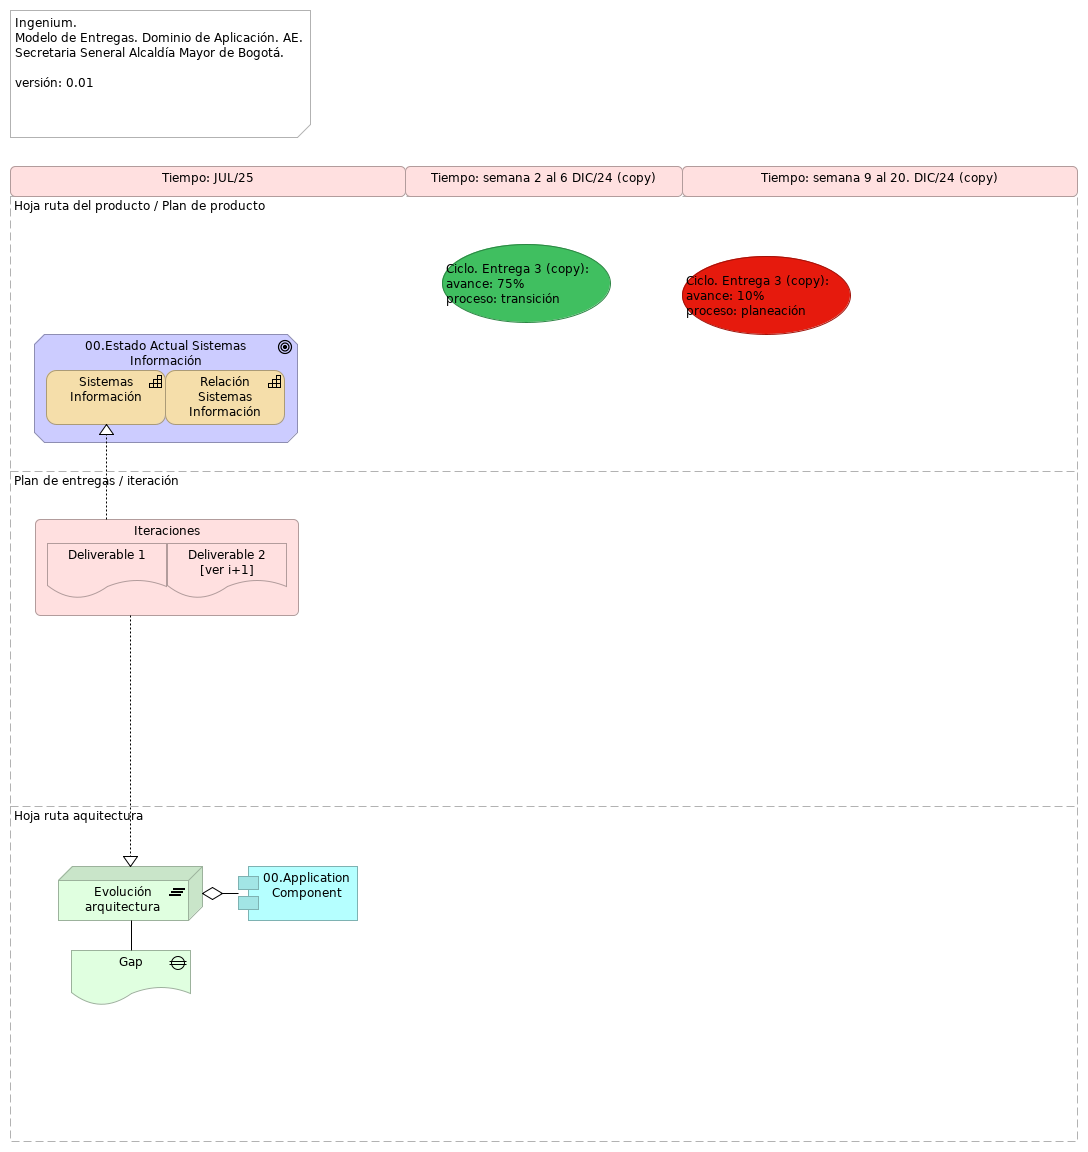
\includegraphics[width=5in,height=\textheight]{images/03.ENTRG.1n.ModelodeEntregas.png}
\caption{03.ENTRG.1n. Modelo de Entregas. \emph{Fuente: Propuesta
servicios de ingeniería y evaluación de arquitectura Arquitectura de
Aplicaciones Secretaria de la Alcaldía de Bogotá
(2025)}}\label{fig:id-b7aa07be1bf34794b7ab18f800fd4d63}
\end{figure}

\subsubsection{Elementos del Modelo}\label{sec:elementos-del-modelo}

\begin{longtable}[]{@{}lll@{}}
\caption{\label{tbl:tblelement-03.ENTRG.1n.ModelodeEntregas-id}Elementos
de la vista.}\tabularnewline
\toprule\noalign{}
Nombre & Tipo & Documentación \\
\midrule\noalign{}
\endfirsthead
\toprule\noalign{}
Nombre & Tipo & Documentación \\
\midrule\noalign{}
\endhead
\bottomrule\noalign{}
\endlastfoot
Hoja ruta del producto / Plan de producto & Grouping & \\
Plan de entregas / iteración & Grouping & \\
Hoja ruta arquitectura & Grouping & \\
\end{longtable}

\subsection{Entregables Fase I de la Visión AE de
SG}\label{sec:entregables-fase-i-de-la-visiuxf3n-ae-de-sg}

\begin{quote}
\end{quote}

\begin{figure}
\centering
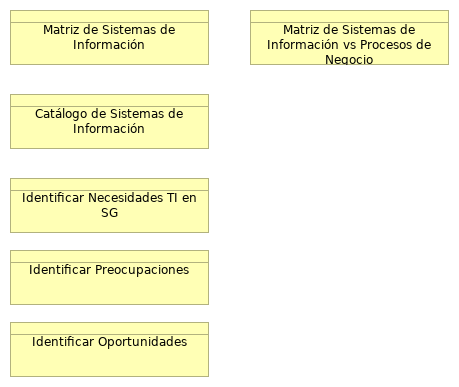
\includegraphics{images/03.EntregablesdelaVision.png}
\caption{03. Entregables de la Vision. \emph{Fuente: Propuesta servicios
de ingeniería y evaluación de arquitectura Arquitectura de Aplicaciones
Secretaria de la Alcaldía de Bogotá
(2025)}}\label{fig:id-0993b3b264144f84abe5c7031666fede}
\end{figure}

\subsubsection{Matriz de Sistemas de
Información}\label{sec:matriz-de-sistemas-de-informaciuxf3n}

Las matrices del dominio de aplicaciones de software y sistemas de
información (SI) de SG son herramientas para el relacionamiento con
otros dominios del ejercicio de arquitectura empresarial de SG. Con esto
conseguimos soportar la toma decisiones de lo que debe ser compartido de
los SI dentro de la Secretaría, y entre sus aplicaciones de software.
Las matrices de este ejercicio sirven además para comunicar el grado de
relacionamiento de los elementos.

En resumen,

\begin{itemize}
\tightlist
\item
  Las matrices son cruciales para especificar cómo debe relacionarse la
  información entre los sistemas y otros dominios
\item
  proporcionan información crítica para los proyectos que involucren a
  los sistemas de SG.
\item
  Contribuye a la determinación de brechas (gaps) en las necesidades de
  compartir información (o funciones de los sistemas) ente los elementos
  de la matriz.
\item
  La matriz ayuda a definir el nivel de detalle de lo que se comparte.
\item
  Se deben establecer medidas similares para la interoperabilidad de
  servicios/negocios y la infraestructura (tecnología física).
\item
  Sintetizan la información de las arquitecturas, y son simples para
  compartir documentos.
\end{itemize}

Las matrices de este dominio (procesos e interoperabilidad) actúan como
una hoja de ruta para la conectividad y el intercambio de información;
inician desde una perspectiva de negocio de alto nivel y van hasta una
especificación técnica detallada del la interacción con los sistemas.
Sirven como herramienta de comunicación para los demás dominios de la
arquitectura empresarial de SG, y contribuyen a que las interacciones
relevantes entre servicios, canales, y procesos estén definidas y sean
compatibles.

\subsubsection{Matriz de Sistemas de Información vs Procesos de
Negocio}\label{sec:matriz-de-sistemas-de-informaciuxf3n-vs-procesos-de-negocio}

Las matrices del dominio de aplicaciones de software y sistemas de
información (SI) de SG son herramientas para el relacionamiento con
otros dominios del ejercicio de arquitectura empresarial de SG. Con esto
conseguimos soportar la toma decisiones de lo que debe ser compartido de
los SI dentro de la Secretaría, y entre sus aplicaciones de software.
Las matrices de este ejercicio sirven además para comunicar el grado de
relacionamiento de los elementos.

En resumen,

\begin{itemize}
\tightlist
\item
  Las matrices son cruciales para especificar cómo debe relacionarse la
  información entre los sistemas y otros dominios
\item
  proporcionan información crítica para los proyectos que involucren a
  los sistemas de SG.
\item
  Contribuye a la determinación de brechas (gaps) en las necesidades de
  compartir información (o funciones de los sistemas) ente los elementos
  de la matriz.
\item
  La matriz ayuda a definir el nivel de detalle de lo que se comparte.
\item
  Se deben establecer medidas similares para la interoperabilidad de
  servicios/negocios y la infraestructura (tecnología física).
\item
  Sintetizan la información de las arquitecturas, y son simples para
  compartir documentos.
\end{itemize}

Las matrices de este dominio (procesos e interoperabilidad) actúan como
una hoja de ruta para la conectividad y el intercambio de información;
inician desde una perspectiva de negocio de alto nivel y van hasta una
especificación técnica detallada del la interacción con los sistemas.
Sirven como herramienta de comunicación para los demás dominios de la
arquitectura empresarial de SG, y contribuyen a que las interacciones
relevantes entre servicios, canales, y procesos estén definidas y sean
compatibles.

\subsubsection{Catálogo de Sistemas de
Información}\label{sec:catuxe1logo-de-sistemas-de-informaciuxf3n}

En el contexto de TOGAF, El Catálogo de sistemas de información es un
inventario detallado y documentado que actúa como ficha técnica de los
sistemas de información o aplicaciones de software de SG.

Es un producto entregable clave de la fase de Arquitectura de
Aplicaciones dentro de la Fase 3 de este ejercicio de arquitectura
empresarial (AE). Forma parte del Marco de Referencia del Contenido
Arquitectónico de TOGAF y del Marco de Arquitectura de Referencia del
MinTIC (MAE 3.0, Colombia).

La construcción del catálogo de aplicaciones implican a las sesiones de
levantamiento, entrevistas, y cuestionarios compartidos en el mes de
julio, junto con la recopilación estructurada de las fuentes de
información sobre cada sistema.

\subsection{Contenido Mínimo del
Catálogo}\label{sec:contenido-muxednimo-del-catuxe1logo}

\begin{itemize}
\tightlist
\item
  ID de Aplicación. Código de identificación de la aplicación de
  software.
\item
  Nombre de la Aplicación. Nombre de identificación de la aplicación de
  software.
\item
  Descripción. Funcionamiento básico de la aplicación de software.
\item
  Estado: {[}En producción, en desmantelamiento, en implementación,
  Inactiva{]}
\item
  Categoría: {[}Sistema de apoyo al negocio (misional), herramienta de
  gestión, Ofimática, Seguridad{]}
\item
  Proceso(s) de Negocio Clave(s)
\item
  Capacidad: Capacidades de nivel 2 relacionadas con la aplicación de
  software.
\item
  Tipo de aplicación: Web, Móvil, Cliente Servidor
\item
  Método de despliegue: on-premises, cloud SAAS, cloud PAAS, cloud IAAS
\item
  Tecnología. Aspectos técnicos de la aplicación de software.
\item
  Versión actual de la tecnología
\item
  Responsable técnico en la entidad
\item
  Responsable funcional en la entidad
\item
  Fabricante
\item
  Proveedor de soporte externo
\item
  Fecha de vigencia de soporte externo
\item
  Nombre de servidor. Nombre de red del entorno o nodo contenedor de la
  aplicación de software.
\item
  Criticidad de negocio
\end{itemize}

El Catálogo de aplicaciones de SG procura beneficios estratégicos y
operativos:

\begin{itemize}
\tightlist
\item
  Unifica la documentación y la comunicación: Es un artefacto clave para
  documentar, comprender y comunicar el panorama actual y futuro de las
  aplicaciones.
\item
  Base para la toma de decisiones: Sirve como base para la toma de
  decisiones en la gestión y gobierno de las capacidades de los sistemas
  de SG, y del portafolio y ciclo de vida de las aplicaciones.
\item
  Facilita la actualización continua: Permite la actualización continua
  de las características y atributos relevantes de los sistemas de
  información.
\end{itemize}

\subsubsection{Identificar Necesidades TI en
SG}\label{sec:identificar-necesidades-ti-en-sg}

La construcción de lista de necesidades, preocupaciones y oportunidades
implican a las sesiones de levantamiento, entrevistas, y cuestionarios
compartidos en el mes de julio, junto con la recopilación estructurada
de las fuentes de información sobre cada sistema.

Necesidades de Transformación Digital y Tecnológica La transformación
digital (objetivo estratégico de SG) es un motor fundamental para
alinear las estrategias, procesos y tecnologías de la Secretaría
General. Esta transformación busca:

\begin{itemize}
\item
  Impulsar la transformación digital para alinear estrategias, procesos
  y tecnologías
\item
  (Necesidad) la Modernización y Eficiencia Pública (Driver)
\item
  Cerrar las brechas en la Política de Gobierno Digital, de la cual la
  Arquitectura Empresarial es un habilitador clave.
\item
  Modernizar la infraestructura tecnológica obsoleta para asegurar su
  continuidad y disponibilidad.
\item
  Integrar plataformas y ecosistemas digitales y superar la falta de
  interoperabilidad.
\item
  Automatizar trámites y estandarizar la gestión y gobernanza de datos
  públicos.
\item
  Adquirir software especializado en análisis de datos para mejorar la
  toma de decisiones basada en evidencia.
\item
  Generar análisis predictivos y prospectivos de resultados de gestión,
  que son insumos para la toma de decisiones.
\item
  Contar con disponibilidad de personal adecuado para actualizar
  plataformas tecnológicas y la gstión de las cargas de trabajo es una
  necesidad identificada para este eje.
\item
  Aprovechar nuevas tecnologías como la Inteligencia Artificial, la
  minería de datos, el procesamiento del lenguaje, para mejorar los
  procesos y la relación con la ciudadanía.
\item
  Abordar los altos costos de la tecnología que limitan la
  implementación de sistemas avanzados. (??)
\item
  Fortalecer la ciberseguridad y seguridad de la información para
  proteger la integridad, disponibilidad y confidencialidad de los datos
  y prevenir ataques.
\end{itemize}

Necesidades Específicas del Dominio de Aplicaciones de software Esta
capa se refiere al comportamiento de las aplicaciones que apoyan el
negocio, la estructura de esas aplicaciones y su relación con los
objetos de datos que utilizan.

Para los Componentes de Aplicación (Application Component) y Servicios
de Aplicación (Application Service) de SG:

\begin{itemize}
\tightlist
\item
  Adquirir software especializado en análisis de datos: implica la
  necesidad de incorporar de nuevos componentes de aplicación
  (Application Component).
\item
  Integrar plataformas y ecosistemas digitales :requiere reforzar la
  relación entre componentes de aplicación y la exposición de servicios
  de aplicación (Application Service), y clicar los lineamientos del
  Marco de Referencia de AE, versión 3.0 al momento, del MinTIC.
\item
  Mejorar la capacidad de las herramientas tecnológicas para el soporte
  a la toma de decisiones y la gestión: requiere la mejora de las
  Funcionalidad (Application Function) y Componentes de Aplicación
  actuales asociadas a esta capacidad.
\end{itemize}

\subsubsection{Identificar
Preocupaciones}\label{sec:identificar-preocupaciones}

Con base en el estudio de las sesiones de levantamiento, entrevistas, y
cuestionarios compartidos en el mes de julio, junto con la recopilación
estructurada de las fuentes de información sobre cada sistema,
identificamos las siguientes preocupaciones (y debilidades) de SG
relacionadas con el dominio de sistemas de información, dentro del
alcance de este ejercicio.

\begin{enumerate}
\def\labelenumi{\arabic{enumi}.}
\tightlist
\item
  Deficiente apropiación del conocimiento en procesos de tecnologías de
  la información, lo que genera demora en la solución de los servicios
  de tecnologías de la información {[}2{]}.
\item
  Equipos tecnológicos obsoletos que generan dificultad en la ejecución
  de las actividades que desarrolla la entidad {[}3{]}.
\item
  Fallas recurrentes en el funcionamiento de los sistemas de información
  y plataformas tecnológicas de la entidad, que afectan la continuidad
  del servicio y generan retrasos y reprocesos en la ejecución de las
  actividades {[}4{]}.
\item
  Insuficiencia en la capacidad de las herramientas tecnológicas de la
  entidad que pueden obstaculizar la obtención y descarga de material
  probatorio relevante para el adelantamiento de procesos disciplinarios
  {[}5{]}.
\item
  Falta de un software que le permita a la entidad extraer una
  información dinámica que sirva como insumo para la toma de decisiones
  {[}6{]}.
\item
  Se realizan análisis descriptivos, pero no predictivos y prospectivos
  de los resultados de la gestión de la entidad, lo que dificulta la
  toma de decisiones basada en evidencia {[}7{]}.
\item
  Falta de personal para actualizar las plataformas tecnológicas, lo que
  genera retrasos en la operación de la entidad {[}8{]}.
\item
  Deficiente conectividad y falta de interoperabilidad de las
  plataformas tecnológicas {[}8{]}.
\item
  Cambios en las plataformas tecnológicas que no interactúan con las
  anteriores, generando posibles pérdidas de información y reprocesos
  {[}9{]}.
\item
  La inestabilidad de la conectividad, indisponibilidad de servidores de
  información y vulnerabilidad en la seguridad informática, lo que puede
  comprometer la operatividad, la integridad de los datos críticos de la
  entidad y el cumplimiento de las metas {[}10{]}.
\item
  La vulneración de la inviolabilidad de acceso a cuentas de correo
  institucionales y aplicativos, lo que afecta la reserva de la
  información relacionada con el trámite de procesos disciplinarios
  {[}10{]}.
\item
  Obsolescencia tecnológica que implica la necesidad de renovación de
  los equipos y dificulta la prestación de los servicios de la entidad
  {[}11{]}.
\item
  Los altos costos de la tecnología pueden limitar la capacidad de la
  entidad para implementar y mantener sistemas avanzados y eficientes
  {[}11{]}.
\item
  Materialización de riesgos asociados a ataques cibernéticos, e
  ingeniería social, suplantación de identidad, entre otros, que ponen
  en riesgo la seguridad de la información y los documentos (pérdida de
  la confidencialidad, integridad y disponibilidad de la información) y
  afectan la continuidad operativa {[}12{]}.
\item
  Estas debilidades resaltan la necesidad de modernizar la
  infraestructura y sistemas tecnológicos, mejorar la gestión de datos
  para análisis predictivos, fortalecer la ciberseguridad, y asegurar la
  capacitación y el personal adecuado para la gestión tecnológica
  {[}2-12{]}.
\end{enumerate}

\subsubsection{Identificar
Oportunidades}\label{sec:identificar-oportunidades}

La construcción de lista de oportunidades mencionadas implica el estudio
de las sesiones de levantamiento, entrevistas, y cuestionarios
compartidos en el mes de julio, junto con la recopilación estructurada
de las fuentes de información al respecto de cada sistema de SG.

Fuente: Sección ``10.15.1 Resultado de la gestión de las oportunidades
vigencia 2023'' del documento
``contexto\_estrategico\_-4202000-ot-066-\_v05.pdf'' {[}1-13{]},

Las oportunidades tecnológicas y de mejora de sistemas de información
mencionadas indicadas en estas fuentes se centran en:

\begin{itemize}
\item
  Modernización de la infraestructura y sistemas tecnológicos,

  \begin{itemize}
  \tightlist
  \item
    Las nuevas tecnologías, especialmente la Inteligencia Artificial
    (IA), ofrecen la oportunidad de mejorar los procesos y herramientas
    de relacionamiento con la ciudadanía {[}15{]}. Bogotá ya ha empezado
    a incorporar tecnologías como IA, Big Data e Internet de las Cosas
    (IoT) en la planificación urbana y la prestación de servicios
    {[}16{]}.
  \item
    Una oportunidad es la adquisición de software especializado en
    análisis de datos para la toma de decisiones que ya poseen otras
    entidades {[}17{]}.
  \end{itemize}
\item
  Integración y automatización de procesos,

  \begin{itemize}
  \tightlist
  \item
    Se identifican oportunidades para tener herramientas que evalúen el
    soporte tecnológico personalizado, flexible y configurable para las
    operaciones de los procesos jurídicos {[}26{]}.
  \item
    Se buscan mejores controles e integración del sistema de régimen
    legal de la Secretaría Jurídica {[}27{]}.
  \item
    También se necesitan mejores controles e integración de los sistemas
    de información como, los sistemas GLOBO (de gestión internacional),
    el sistema de proyectos GLPI, entre otros
  \end{itemize}
\item
  Fortalecimiento de la seguridad digital,

  \begin{itemize}
  \tightlist
  \item
    Una oportunidad es la adquisición de software especializado en
    análisis de datos para la toma de decisiones que ya poseen otras
    entidades {[}17{]}.
  \end{itemize}
\item
  Mejora de la comunicación pública a través de medios digitales,

  \begin{itemize}
  \tightlist
  \item
    Se busca la consolidación de herramientas, canales e información
    para fortalecer la oferta y celeridad de servicios y la
    participación ciudadana {[}11{]}. Esto incluye el seguimiento a
    canales de atención virtual como SuperCADE Virtual, chat, chat-Bot y
    videollamadas de la línea 195 {[}11{]}.
  \item
    Se busca optimizar los procesos de recolección, análisis y
    divulgación de la información mediante la implementación de sistemas
    de información que contengan la automatización de la recolección de
    datos y el uso de herramientas analíticas {[}15{]}.
  \item
    Una noticia reciente destaca que el Distrito unifica en el portal
    Bogotá su oferta de trámites y servicios, el cual permite acceder a
    más de 1.400 trámites y servicios y realizar pagos en línea (no
    tributarios) y agendamiento de citas en la RedCADE desde casa
    {[}40{]}. Esto representa una mejora significativa en la
    accesibilidad y eficiencia de los servicios digitales para la
    ciudadanía.
  \end{itemize}
\item
  Capacitación en nuevas tecnologías (\ldots).
\item
  Implementación de la Arquitectura Empresarial como estrategia para
  impulsar la transformación digital y la eficiencia en la gestión
  pública de la SG.

  \begin{itemize}
  \tightlist
  \item
    Se espera que la Arquitectura Empresarial fortalezca la
    transparencia y rendición de cuentas al estandarizar procesos y
    sistemas de información, aumentando la confianza de la ciudadanía en
    la Gestión Pública {[}25{]}.
  \item
    Es requerido que este ejercicio beneficie a la SG con la entrega de
    activos como hojas de ruta, catálogos y caracterización de los
    sistemas de información, matrices de interacción, entre otros.
  \end{itemize}
\end{itemize}\sidenote{This is a sidenote. This template features a large margin specifically so you can put notes, figures, tables and other things into it as additional material to the main content in the text block.}

Donec in elit ac ante vestibulum rhoncus. Pellentesque ligula tortor, aliquet malesuada nulla tristique vitae. Aliquam mi sem, varius eu pellentesque et, tristique nec quam. Vestibulum pellentesque in dui et venenatis. Sed malesuada elit pellentesque sapien aliquet porta. In at facilisis diam. Duis id ante tellus.\sidenote[][2cm]{This sidenote has been pushed down the page manually with an optional parameter, otherwise it would be right under the one above.} % This first optional argument to a sidenote is the symbol to use (leave this empty for automatic numbering) and the second is the vertical offset (positive is down, negative is up)

In diam libero, vulputate quis accumsan non, auctor in ipsum. Praesent cursus velit eget lacus sodales porta. Proin quis risus ut velit euismod scelerisque ut sed neque. Cras sagittis, dolor ac ullamcorper auctor, tortor dui facilisis diam, at sagittis nisi ipsum a neque. Nullam vel mattis nisi. Ut interdum ut diam at ornare. Nulla ultrices elit justo, vitae tristique massa vulputate sit amet.

\nonumsidenote{
	}Vestibulum erat felis, cursus vitae convallis ac, commodo eu nisi. Nulla facilisi. Mauris dignissim nisi felis, a mollis ex accumsan vel. Suspendisse bibendum vitae nibh in suscipit. Vestibulum et finibus eros. Nulla facilisi. Cras luctus aliquam finibus. In nec justo nec orci malesuada faucibus.

\subsubsection{Subsubsection Title} % Third level section

\begin{fullwidth} % Use the whole page width
	\textit{This is an example of a full width paragraph\ldots} Curabitur id placerat orci. Vivamus pulvinar augue ac feugiat blandit. Donec in ultricies mi. Nam eu lacus ac augue aliquet consectetur. Praesent dui risus, sollicitudin nec felis ut, posuere ultricies dolor. Sed massa nulla, dignissim eget sem sit amet, eleifend fermentum dui. Phasellus consequat sem vel turpis finibus, a aliquam risus malesuada.
\end{fullwidth}

Maecenas consectetur metus at tellus finibus condimentum. Proin arcu lectus, ultrices non tincidunt et, tincidunt ut quam. Integer luctus posuere est, non maximus ante dignissim quis. Nunc a cursus erat. Curabitur suscipit nibh in tincidunt sagittis. Nam malesuada vestibulum quam id gravida. Proin ut dapibus velit. Vestibulum eget quam quis ipsum semper convallis. Duis consectetur nibh ac diam dignissim, id condimentum enim dictum. Nam aliquet ligula eu magna pellentesque, nec sagittis leo lobortis. Aenean tincidunt dignissim egestas. Morbi efficitur risus ante, id tincidunt odio pulvinar vitae.

\paragraph{Paragraph Title} % Fourth level section

Lorem ipsum dolor sit amet, consectetur adipiscing elit. Aliquam auctor mi risus, quis tempor libero hendrerit at. Duis hendrerit placerat quam et semper. Nam ultricies metus vehicula arcu viverra, vel ullamcorper justo elementum. Pellentesque vel mi ac lectus cursus posuere et nec ex.

The section titles below show how multi-line section titles look at the 3 top levels.


%----------------------------------------------------------------------------------------
%	QUOTATIONS
%----------------------------------------------------------------------------------------

\section{Quotations}

Proin mollis urna posuere fringilla. Curabitur finibus, neque vitae vestibulum vestibulum, dolor sapien tincidunt augue, vel porta mauris metus nec mauris. Integer erat magna, porta id erat sed, lacinia volutpat erat. Nulla fermentum tellus arcu, eu iaculis ipsum malesuada aliquam. Duis et lacus maximus, consectetur metus et, eleifend arcu. Vestibulum condimentum diam vitae diam tincidunt viverra.\sidenotequote[-1cm]{\textbf{\LARGE ``}Lorem ipsum dolor sit amet, consectetur adipiscing elit. Praesent porttitor arcu luctus, imperdiet urna iaculis, mattis eros. Pellentesque iaculis odio vel nisl ullamcorper, nec faucibus ipsum molestie.\textbf{''}\\[4pt]\hfill--- John Smith, 1972} % Example margin quotation using the \sidenotequote custom command

\begin{quote}
	\textbf{\LARGE ``}Lorem ipsum dolor sit amet, consectetur adipiscing elit. Praesent porttitor arcu luctus, imperdiet urna iaculis, mattis eros. Pellentesque iaculis odio vel nisl ullamcorper, nec faucibus ipsum molestie. Sed dictum nisl non aliquet porttitor. Etiam vulputate arcu dignissim, finibus sem et, viverra nisl. Aenean luctus congue massa, ut laoreet metus ornare in.\textbf{''}
	
	\hfill--- John Smith, 1972
\end{quote}

Suspendisse tempus odio sit amet volutpat suscipit. Pellentesque ornare libero lacus, non fringilla dolor placerat in. Ut maximus ullamcorper lectus, a pharetra mi sagittis aliquet. Scelerisque augue sed mi fringilla, vel dapibus ligula finibus. Sed ornare velit sem, ac venenatis velit dignissim. Vestibulum ultrices mi at tincidunt condimentum.

%----------------------------------------------------------------------------------------
%	TABLES
%----------------------------------------------------------------------------------------

\section{Table Examples}

This statement automatically references the table below using its label: Table \ref{tab:example}.

%------------------------------------------------

\begin{margintable} % Use the margintable environment for tables to be output to the margin
	\footnotesize % Reduce the font size in the table as space is at a premium
	\caption{Margin table caption.}
	\begin{tabular}{L{0.22\linewidth} C{0.22\linewidth} R{0.25\linewidth}}
		\toprule
		\textbf{Year} & \textbf{Qtr.} & \textbf{Perf.}\\
		\midrule
		20XX & Q1 & 0.5\%\\
		20XX & Q2 & 26.5\%\\
		20XX & Q1 & 35.4\%\\
		20XX & Q4 & 41.3\%\\
		\bottomrule
	\end{tabular}
\end{margintable}

%------------------------------------------------

\begin{table}[H] % [H] forces the table to be output where it is defined in the code (it suppresses floating)
	\caption{Text block table caption.}
	\begin{tabular}{L{0.35\linewidth} L{0.38\linewidth} L{0.16\linewidth}}
		\toprule
		\textbf{Prospect} & \textbf{Industry} & \textbf{Revenue} \\
		\midrule
		Gerlach Inc & Business Development & 3M\\
		Doyle and Sons & Law & 1M\\
		Heathcote Group & Consulting & 12M\\
		Goyette Inc & Advertising & 5M\\
		Holzdeppe GmbH & Manufacturing & 23M\\
		Bienias AG & Accounting & 2.5M\\
		\bottomrule
	\end{tabular}
	\label{tab:example}
\end{table}

%------------------------------------------------

\begin{table*} % Use the table* environment for full width tables
	\caption{Full width table caption.}
	\begin{tabular}{C{0.03\linewidth} L{0.25\linewidth} L{0.27\linewidth} L{0.16\linewidth} L{0.16\linewidth}}
		\toprule
		\textit{\#} & \textbf{Prospect} & \textbf{Industry} & \textbf{Revenue} & \textbf{Employees} \\
		\midrule
		\textit{1} & Gerlach Inc & Business Development & 3M & 65\\
		\textit{2} & Doyle and Sons & Law & 1M & 15\\
		\textit{3} & Heathcote Group & Consulting & 12M & 250\\
		\textit{4} & Goyette Inc & Advertising & 5M & 100\\
		\textit{5} & Holzdeppe GmbH & Manufacturing & 23M & 75\\
		\textit{6} & Bienias AG & Accounting & 2.5M & 40\\
		\bottomrule
	\end{tabular}
\end{table*}

%----------------------------------------------------------------------
%	FIGURES
%----------------------------------------------------------------------

\section{Figure Examples}

This statement automatically references the figure below using its label: Figure \ref{fig:example}.

%------------------------------------------------

\begin{marginfigure} % Use the marginfigure environment for figures to be output to the margin
	
\includegraphics[width=\linewidth]{./include/placeholder.jpg}
	\caption{Margin figure caption.}
\end{marginfigure}

%------------------------------------------------

\begin{figure}[H] % [H] forces the figure to be output where it is defined in the code (it suppresses floating)
	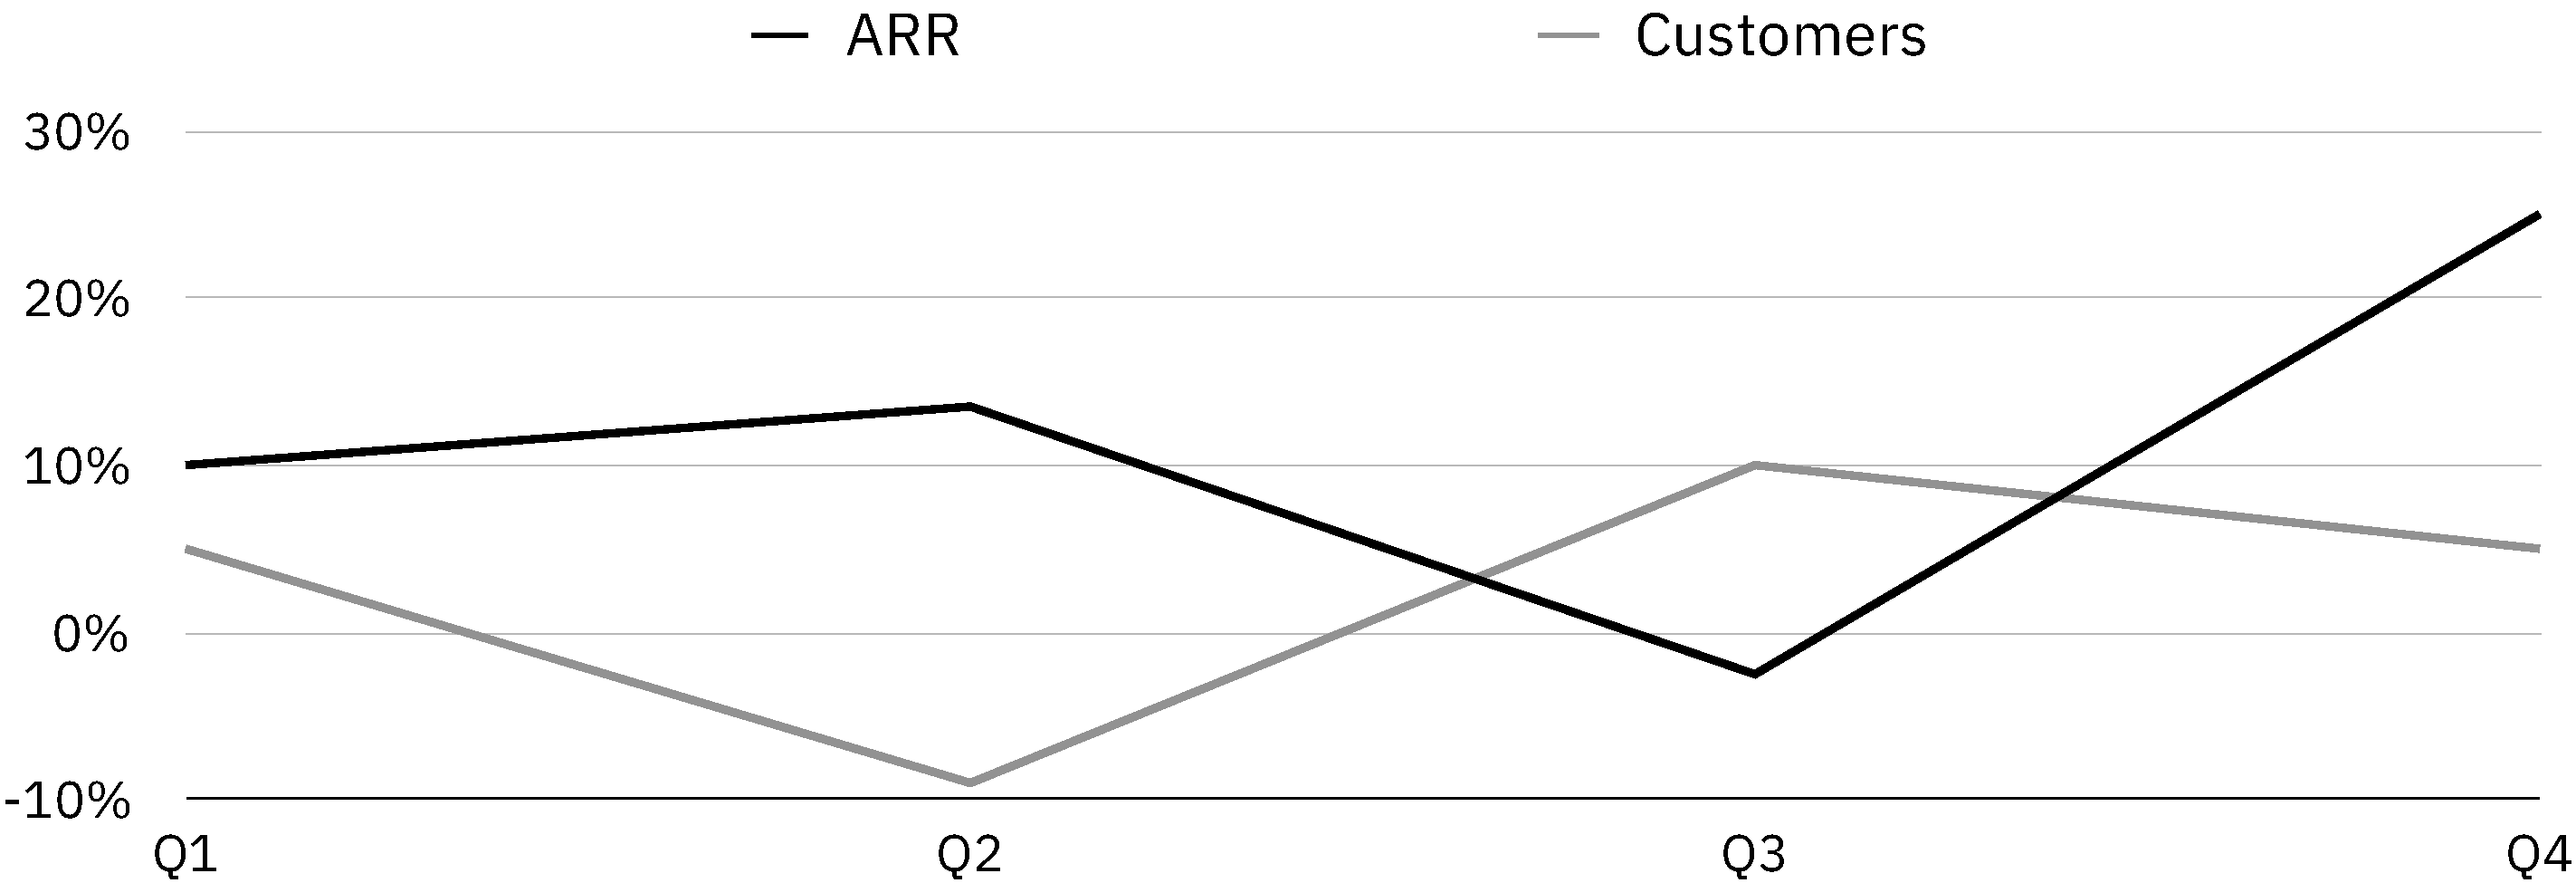
\includegraphics[width=\linewidth]{./include/ARR.pdf}
	\caption{Text block figure caption.}
	\label{fig:example} % Label for referencing this figure in the text automatically
\end{figure}

%------------------------------------------------

\begin{figure*} % Use the figure* environment for full width figures
	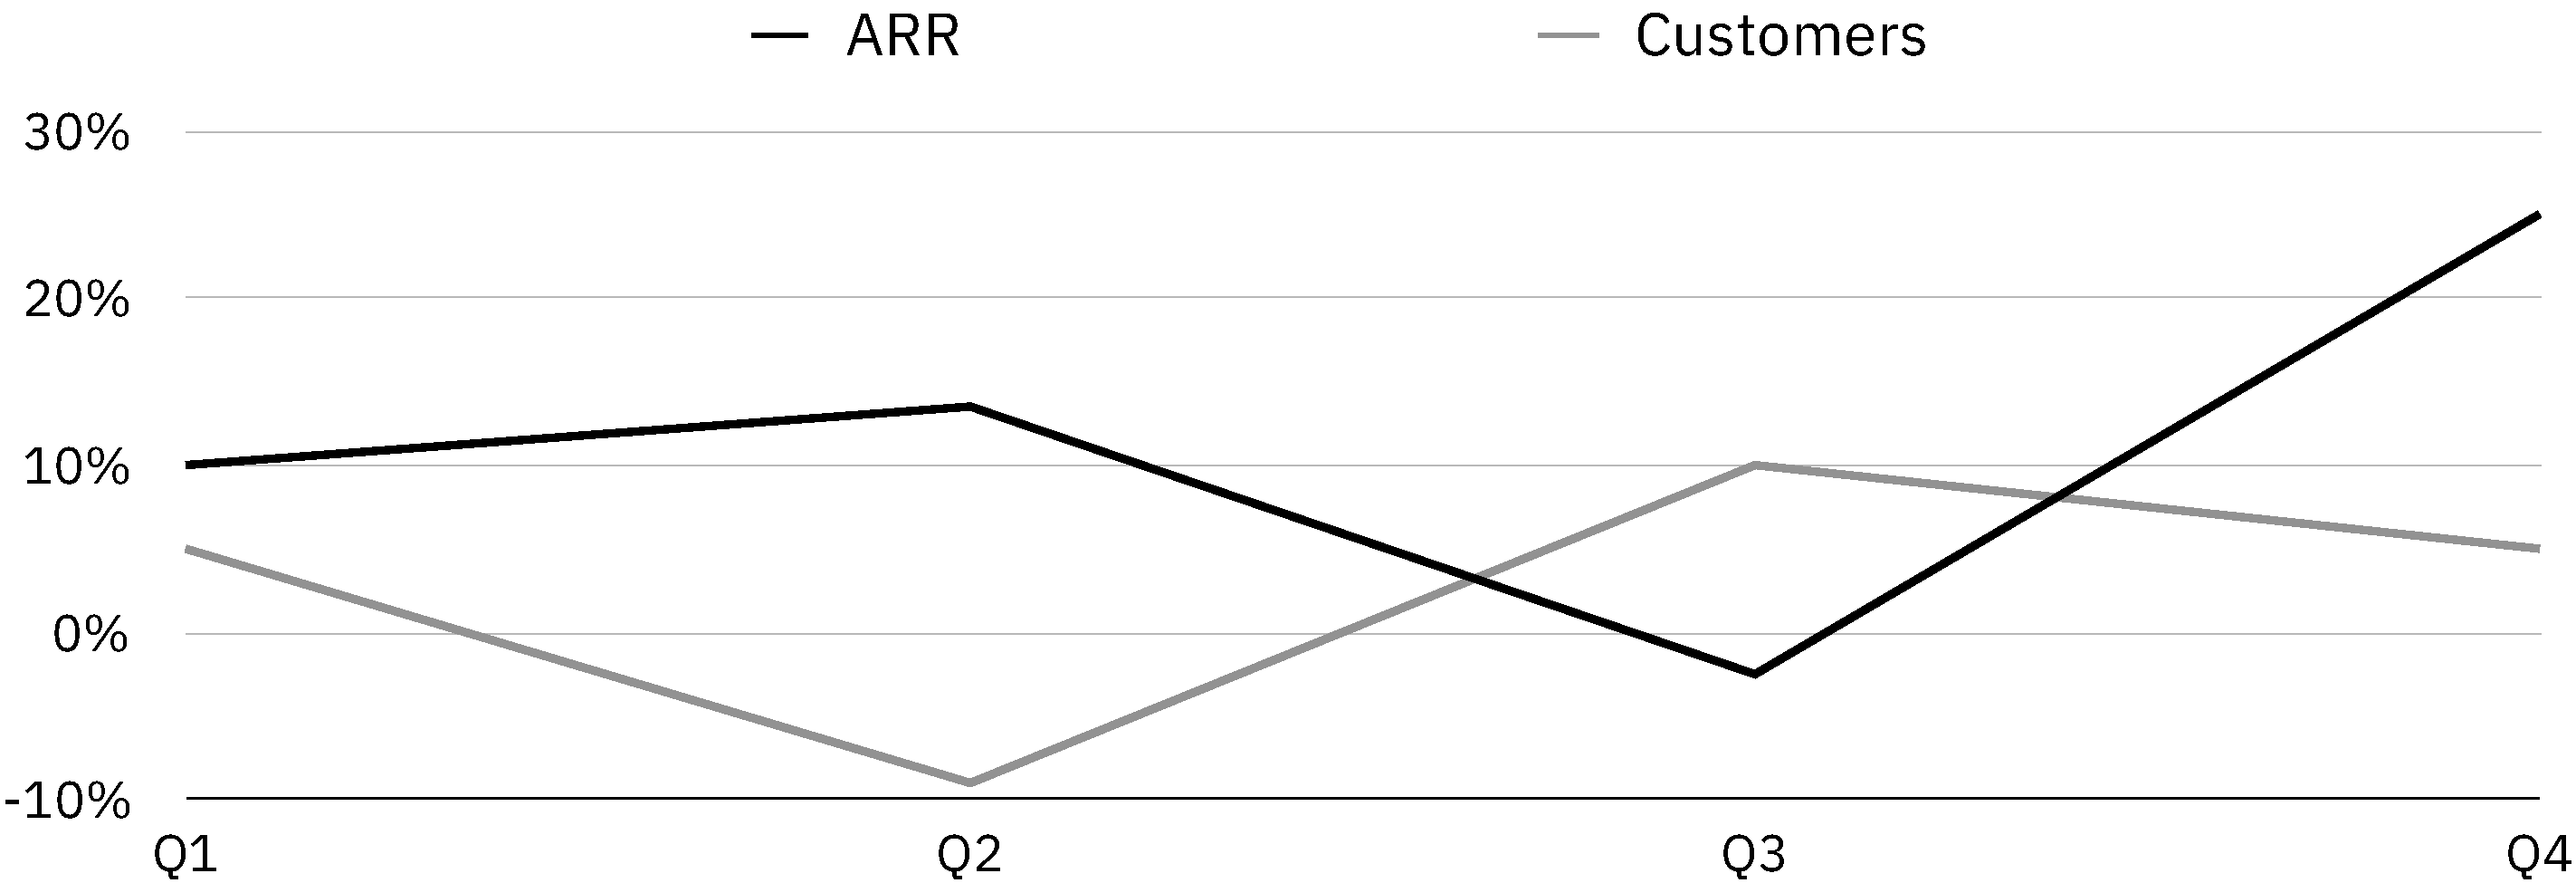
\includegraphics[width=\linewidth]{./include/ARR.pdf}
	\caption{Full width figure caption.}
\end{figure*}

%----------------------------------------------------------------------------------------
%	LISTS
%----------------------------------------------------------------------------------------

\section{List Examples}

\subsection{Bullet Point List}

\nonumsidenote{Bullet point lists can also be created in the margin. For these, we can remove the usual left margin to increase the available horizontal space:\\\medskip \begin{itemize}[leftmargin=*]\item Bullet item one. \item Bullet item two. \item Bullet item three.\end{itemize}}Lorem ipsum dolor sit amet, consectetur adipiscing elit. Praesent porttitor arcu luctus, imperdiet urna iaculis, mattis eros. Pellentesque iaculis odio vel nisl ullamcorper, nec faucibus ipsum molestie. Sed dictum nisl non aliquet porttitor.

\begin{itemize}
	\item First bullet point item
	\begin{itemize}
		\item First indented bullet point item
		\item Second indented bullet point item
		\begin{itemize}
			\item First second-level indented bullet point item
			\item Second second-level indented bullet point item
		\end{itemize}
		\item Third indented bullet point item
	\end{itemize}
	\item Second bullet point item
	\item Third bullet point item
\end{itemize}

Etiam vulputate arcu dignissim, finibus sem et, viverra nisl. Aenean luctus congue massa, ut laoreet metus ornare in. Nunc fermentum nisi imperdiet lectus tincidunt vestibulum at ac elit. Nulla mattis nisl eu malesuada suscipit.

%------------------------------------------------

\subsection{Numbered List}

\nonumsidenote[-2.5cm]{Numbered lists can also be created in the margin. For these, we can remove the usual left margin to increase the available horizontal space:\\\medskip \begin{enumerate}[leftmargin=*]\item Numbered item one. \item Numbered item two. \item Numbered item three.\end{enumerate}}Lorem ipsum dolor sit amet, consectetur adipiscing elit. Praesent porttitor arcu luctus, imperdiet urna iaculis, mattis eros. Pellentesque iaculis odio vel nisl ullamcorper, nec faucibus ipsum molestie. Sed dictum nisl non aliquet porttitor.

\begin{enumerate}
	\item First numbered item
	\begin{enumerate}
		\item First indented numbered item
		\item Second indented numbered item
		\begin{enumerate}
			\item First second-level indented numbered item
			\item Second second-level indented numbered item
		\end{enumerate}
		\item Third indented numbered item
	\end{enumerate}
	\item Second numbered item
	\item Third numbered item
\end{enumerate}

Etiam vulputate arcu dignissim, finibus sem et, viverra nisl. Aenean luctus congue massa, ut laoreet metus ornare in. Nunc fermentum nisi imperdiet lectus tincidunt vestibulum at ac elit. Nulla mattis nisl eu malesuada suscipit.

%------------------------------------------------

\subsection{Description List}

\nonumsidenote{Description lists can also be created in the margin:\\\medskip \begin{description}\item[A1] Description item one. \item[B1] Description item two. \item[C1] Description item three.\end{description}}Lorem ipsum dolor sit amet, consectetur adipiscing elit. Praesent porttitor arcu luctus, imperdiet urna iaculis, mattis eros. Pellentesque iaculis odio vel nisl ullamcorper, nec faucibus ipsum molestie. Sed dictum nisl non aliquet porttitor.

\begin{description}
	\item[Item One] Lorem ipsum dolor sit amet, consectetur adipiscing elit. Praesent porttitor arcu luctus, imperdiet urna iaculis, mattis eros. Pellentesque iaculis odio vel nisl ullamcorper, nec faucibus ipsum molestie.
	\item[Item Two] Sed dictum nisl non aliquet porttitor.
	\begin{description}
		\item[Subitem] Maecenas consectetur metus at tellus finibus condimentum. Proin arcu lectus, ultrices non tincidunt et, tincidunt ut quam. Integer luctus posuere est, non maximus ante dignissim quis.
		\begin{description}
			\item[Subsubitem] Maecenas consectetur metus at tellus finibus condimentum. Proin arcu lectus, ultrices non tincidunt et, tincidunt ut quam. Integer luctus posuere est, non maximus ante dignissim quis.
	\end{description}
	\end{description}
	\item[Item Three] Etiam vulputate arcu dignissim, finibus sem et, viverra nisl. Aenean luctus congue massa, ut laoreet metus ornare in. Nunc fermentum nisi imperdiet lectus tincidunt vestibulum at ac elit. Nulla mattis nisl eu malesuada suscipit.
\end{description}

Etiam vulputate arcu dignissim, finibus sem et, viverra nisl. Aenean luctus congue massa, ut laoreet metus ornare in.

%----------------------------------------------------------------------------------------
%	REFERENCING CITATIONS
%----------------------------------------------------------------------------------------

\section{Referencing Citations}

This statement requires citation \autocite{Smith:2024jd}.

This statement requires multiple citations \autocite{Smith:2024jd, Smith:2023qr}.

This short citation is in the margin\sidecite{Smith:2023qr}.

This long citation is in the margin\fullsidecite{Smith:2024jd}.

This statement has an in-text citation: \textcite{Smith:2024jd}.

%----------------------------------------------------------------------------------------
%	LINKS
%----------------------------------------------------------------------------------------

\section{Link Examples}

This is a URL link: \href{https://www.duckduckgo.com}{DuckDuckGo}.\nonumsidenote{Links can be clicked in the PDF to navigate to the linked website or email address.}

This is a email link: \href{mailto:example@example.com}{example@example.com}.

This is a monospaced URL link: \url{https://duckduckgo.com}.


%----------------------------------------------------------------------------------------
%	CODE
%----------------------------------------------------------------------------------------

\section{Displaying Code}

The block below is a code listing. It displays code in an easy to use way with line numbers for quick reference to specific parts of the code.

\begin{lstlisting}
{
	"city": [
		{
			"id": 1,
			"name": "Toronto",
			"country": "Canada",
			"population": 6200000
		},
		{
			"id": 2,
			"name": "New York",
			"country": "United States of America",
			"population": 8800000
		}
	]
}
\end{lstlisting}

%----------------------------------------------------------------------------------------
%	 REFERENCES/BIBLIOGRAPHY
%----------------------------------------------------------------------------------------

\newpage

\addcontentsline{toc}{section}{Reference List} % Add the bibliography to the table of contents

\begin{twothirdswidth} % Content in this environment to be at two-thirds of the whole page width
	\printbibliography[title=Reference List] % Output the bibliography with a custom section title
\end{twothirdswidth}

%----------------------------------------------------------------------------------------
%	APPENDICES
%----------------------------------------------------------------------------------------

\newpage

\section*{Appendices}

\begin{appendices}

\section{Appendix Section}

Lorem ipsum dolor sit amet, consectetur adipiscing elit. Aliquam auctor mi risus, quis tempor libero hendrerit at. Duis hendrerit placerat quam et semper. Nam ultricies metus vehicula arcu viverra, vel ullamcorper justo elementum. Pellentesque vel mi ac lectus cursus posuere et nec ex. Fusce quis mauris egestas lacus commodo venenatis. Ut at arcu lectus. Donec et urna nunc. Morbi eu nisl cursus sapien eleifend tincidunt quis quis est. Donec ut orci ex. Praesent ligula enim, ullamcorper non lorem a, ultrices volutpat dolor. Nullam at imperdiet urna. Pellentesque nec velit eget euismod pretium.

\section{Appendix Section}

Lorem ipsum dolor sit amet, consectetur adipiscing elit. Aliquam auctor mi risus, quis tempor libero hendrerit at. Duis hendrerit placerat quam et semper. Nam ultricies metus vehicula arcu viverra, vel ullamcorper justo elementum. Pellentesque vel mi ac lectus cursus posuere et nec ex. Fusce quis mauris egestas lacus commodo venenatis. Ut at arcu lectus. Donec et urna nunc. Morbi eu nisl cursus sapien eleifend tincidunt quis quis est. Donec ut orci ex. Praesent ligula enim, ullamcorper non lorem a, ultrices volutpat dolor. Nullam at imperdiet urna. Pellentesque nec velit eget euismod pretium.

\section{Appendix Section}

Lorem ipsum dolor sit amet, consectetur adipiscing elit. Aliquam auctor mi risus, quis tempor libero hendrerit at. Duis hendrerit placerat quam et semper. Nam ultricies metus vehicula arcu viverra, vel ullamcorper justo elementum. Pellentesque vel mi ac lectus cursus posuere et nec ex. Fusce quis mauris egestas lacus commodo venenatis. Ut at arcu lectus. Donec et urna nunc. Morbi eu nisl cursus sapien eleifend tincidunt quis quis est. Donec ut orci ex. Praesent ligula enim, ullamcorper non lorem a, ultrices volutpat dolor. Nullam at imperdiet urna. Pellentesque nec velit eget euismod pretium.

\end{appendices}

%----------------------------------------------------------------------------------------

\end{document}
